% This file was created by matlab2tikz.
% Minimal pgfplots version: 1.3
%
%The latest updates can be retrieved from
%  http://www.mathworks.com/matlabcentral/fileexchange/22022-matlab2tikz
%where you can also make suggestions and rate matlab2tikz.
%
\documentclass[tikz]{standalone}
\usepackage{pgfplots}
\usepackage{grffile}
\pgfplotsset{compat=newest}
\usetikzlibrary{plotmarks}
\usepackage{amsmath}

\begin{document}
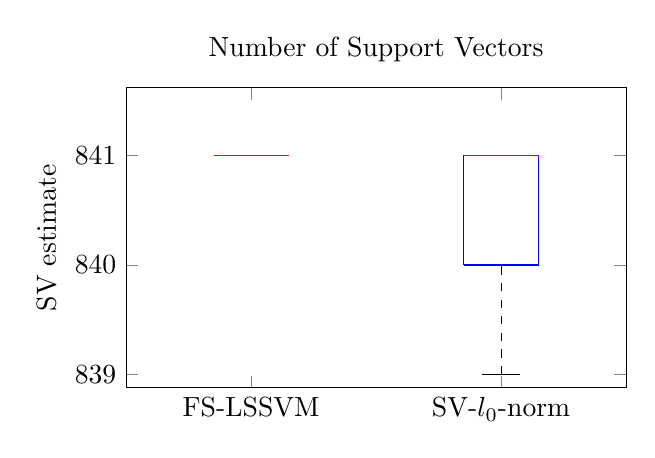
\begin{tikzpicture}

\begin{axis}[%
width=2.5in,
height=1.5in,
scale only axis,
unbounded coords=jump,
xmin=0.5,
xmax=2.5,
xtick={1,2},
ymin=838.875176120368,
ymax=841.621301472279,
ylabel={SV estimate},
xticklabels={{FS-LSSVM},{SV-$l_0$-norm}},
title={Number of Support Vectors}
]
\addplot [color=black,dashed,forget plot]
  table[row sep=crcr]{%
1	841\\
1	841\\
};
\addplot [color=black,dashed,forget plot]
  table[row sep=crcr]{%
2	841\\
2	841\\
};
\addplot [color=black,dashed,forget plot]
  table[row sep=crcr]{%
1	841\\
1	841\\
};
\addplot [color=black,dashed,forget plot]
  table[row sep=crcr]{%
2	839\\
2	840\\
};
\addplot [color=black,solid,forget plot]
  table[row sep=crcr]{%
0.925	841\\
1.075	841\\
};
\addplot [color=black,solid,forget plot]
  table[row sep=crcr]{%
1.925	841\\
2.075	841\\
};
\addplot [color=black,solid,forget plot]
  table[row sep=crcr]{%
0.925	841\\
1.075	841\\
};
\addplot [color=black,solid,forget plot]
  table[row sep=crcr]{%
1.925	839\\
2.075	839\\
};
\addplot [color=blue,solid,forget plot]
  table[row sep=crcr]{%
0.85	841\\
0.85	841\\
1.15	841\\
1.15	841\\
0.85	841\\
};
\addplot [color=blue,solid,forget plot]
  table[row sep=crcr]{%
1.85	840\\
1.85	841\\
2.15	841\\
2.15	840\\
1.85	840\\
};
\addplot [color=red,solid,forget plot]
  table[row sep=crcr]{%
0.85	841\\
1.15	841\\
};
\addplot [color=red,solid,forget plot]
  table[row sep=crcr]{%
1.85	841\\
2.15	841\\
};
\addplot [color=black,only marks,mark=+,mark options={solid,draw=red},forget plot]
  table[row sep=crcr]{%
nan	nan\\
};
\addplot [color=black,only marks,mark=+,mark options={solid,draw=red},forget plot]
  table[row sep=crcr]{%
nan	nan\\
};
\end{axis}
\end{tikzpicture}%
\end{document}